\documentclass[oneside]{book}

\input{\string~/texrc.tex}

\makeatletter

\makeatother

\geometry{tmargin=2cm, bmargin=2cm, lmargin=2cm, rmargin=3cm}

\def\equalwith{\quad$\Longleftrightarrow$\quad}


\begin{document}

\frontmatter

\tableofcontents

\mainmatter

\chapter{开始使用}

%{{{ sec:基本格式
\section{基本的格式}

\subsection{\mpost 示例}

\begin{mpostcode}[code:exmple]
beginfig(1);
u=1cm;
draw origin -- (u, u);
endfig;

end
\end{mpostcode}

\keyword{\lstinline$beginfig(1)$}用于开始一个新的图形, 其中的“1”称为\constant{charcode}, 图形以\keyword{\lstinline$endfig$}结束。\index{Cons-charcode}%
\constant{origin}表示原点{\bf(0, 0)}。使用{\bf mpost}编译以上代码将生成%
以源文件名(\constant{jobname})为前缀\constant{charcode}后缀的\emph{eps}文件。
\index{Cons-jobname}

\subsection{三个内置变量}

\begin{table}{H}
    \centering
    \begin{tabular}{l | l}
        \hline
        {\bf\large prologues} & 用于决定编译器选择PostScript字体, [0, 3]\cr
        \hline
        {\bf\large outputtemplate} & 输出文件的模板\cr
        \hline
        {\bf\large outputformat} & 输出文件的格式\cr
        \hline
    \end{tabular}
    \caption{三个内置变量}
    \label{tab:outputinternal}
\end{table}

\subsubsection{outputtemplate}

输出文件的模板, 为字符串内置变量。模板包含转义字符{\bf \%\{charcode\}}:\newline
\begin{table}{H}
    \centering
    \begin{tabular}{c | l}
        \hline
        {\bf\large \%j} & jobname\cr
        \hline
        {\bf\large \%c} & beginfig的计数\cr
        \hline
        {\bf\large \%\%} & \%字符\cr
        \hline
        {\bf\large \%\{y | m | d | H | M\}} & 一次表示年, 月, 日, 小时,分钟\cr
        \hline
    \end{tabular}
    \caption{转义字符}
    \label{tab:escapechar}
    \index{转义字符}
\end{table}

\subsubsection{outputformat}

字符串内置变量,输出文件的格式,默认为{\bf eps}, 可选为{\bf eps, svg, png}。

\subsubsection{\mpost 文件输出示例}

\begin{mpostcode}[code:example2]
outputformat:="eps";
outputtemplate:="%j-%c.eps";
prologues:=3;

beginfig(1);
u=1cm;
draw origin -- (u, u);
endfig;

end
\end{mpostcode}

编译文件输出{\bf \{jobname\}-1.eps}。
%}}} end sec:基本格式

%{{{ sec:赋值和推断
\section{赋值和推断}

\subsection{赋值}

\mpost 中的赋值符号是{\bf :=},如给内置变量赋值需要使用\expression{\lstinline$<internalVar>:=<value>$}的形式。{\bf :=}的%
右边只能是确定的值,左边是一个变量。

\subsection{推断}

\mpost 中支持线性表达式值的推断,线性表达式的中使用{\bf =},{\bf =}的左右可以互换。例:

\begin{mpostcode}[code:xianxing]
outputformat:="eps";
outputtemplate:="%j-%c.eps";
prologues:=3;

beginfig(1);
    u = 2cm;
    z1 = (x2 + 2u, y3);
    z2 + z3 = (u, 2u);
    z3 - z2 = (0.5u, u);
    draw z1 -- z2 -- z3 --cycle;
endfig;

end
\end{mpostcode}

无名变量线性推断{\color{red}whatever}
\begin{mpostcode}[code:whatever]
outputformat:="eps";
outputtemplate:="%j-%c.eps";
prologues:=3;

beginfig(1);
    u = 2cm;
    z1 = whatever[origin, (2u, 3u)];
    z1 = whatever[(0, 2u), (2u, 0)];
    draw origin -- z1;
endfig;

end
\end{mpostcode}

将{\color{red} whatever}改为其他的变量一样可以。

\section{单位}

\begin{table}[H]
    \centering
    \begin{tabular}{ c | l}
        \hline
        单位 & Explanation\cr
        \hline
        bp & One PostScript point in bp units\cr
        \hline
        cc & One cicero in bp units [12.79213]\cr
        \hline
        cm & One centimeter in bp units [28.34645]\cr
        \hline
        dd & One didot point in bp units [1.06601]\cr
        \hline
        in & One inch in bp units[72]\cr
        \hline
        mm & One millimeter in bp units [2.83464]\cr
        \hline
        pc & One pica in bp units [11.95517]\cr
        \hline
        pt & One printer’s point in bp units [0.99626]\cr
        \hline
    \end{tabular}
    \index{单位}
    \label{tab:units}
    \caption{单位}
\end{table}

所有的单位都会换算成\unit{bp}进行运算, 如\expression{show 1cm * 1cm}会在编译终端显示\disnumber{803.52127}
%}}} end sec:赋值和推断


\chapter{Type}
\index{Type}

变量类型\type{boolean,numeric,pair,path,pen,picture,string,transform}
,还有颜色类型\colortype{rgbcolor,cmykcolor,color}

%{{{ sec:声明
\section{声明}

使用\expression{<type> <var>;}的形式声明变量\expression{<var>}。\par

如\expression{\lstinline$pair m;$},\expression{\lstinline$numeric a;$},%
\expression{\lstinline$string name;$}。

\subsection{newinternal}

使用{\color{blue}\bf newinternal}关键字可以声明新的内置变量,内置变量只可以%
使用{\bf ":="}改变值。
%}}} end sec:声明

%{{{ sec:数组
\section{数组}
\index{Type-array}

\mpost 的数组不声明长度,
声明形如\lstinline$pair pp[];$声明{\bf pp}数组,可以以{\bf pp1,pp2,pp3}%
或者{\bf pp[i]}的形式的调用。
还可以\lstinline$pair p[]p[];$形式的声明,以{\bf p1p1,p1p[i],p.1p.1,p[1]p[1] $\dots$}的形式调用。
%}}} end sec:数组

%{{{ sec:boolean
\section{boolean}
\index{Type-boolean}

\type{boolean}有两个值\constant{true,false},\type{boolean}类型的值由\other{boolean expression}表示。\par
\other{boolean expression}参见\ref{sec:BoolExpression}。
%}}} end sec:boolean

%{{{ sec:numeric
\section{numeric}
\index{Type-numeric}
\label{type:numeric}

%}}} end sec:numeric

%{{{ sec:pair
\section{pair}
\index{Type-pair}
\label{sec:pair}

%}}} end sec:pair

%{{{ sec:path
\section{path}
\index{Type-path}
\label{sec:path}

%}}}

%{{{ sec:pen
\section{pen}
\index{Type-pen}
\label{sec:pen}

%}}} end sec:pen

%{{{ sec:picture
\section{picture}

\subsection{thelabel}
\index{Macro-thelabel}

使用\macro{thelabel}可以返回一个\type{picture}。如\expression{pp = thelabel.bot(%
"Hello world!",origin)}返回\constant{pp},使用\expression{show pp}可以将其打印出来。

\macro{thelabel}的形式:\newline
\indent \expression{thelabel.<suffix>(string | picture,point)}\par

\noindent\lstinline$<suffix>$:\quad{\bf top,bot,lft,rt,ulft,llft,urt,lrt}

与\macro{thelabel}相关的两个宏\macro{label}、\macro{dotlabel}都直接将\type{picture}打印出来。

\subsubsection{thelabel示例}

\begin{mpostcode}[code:thelabel]
outputformat:="eps";
outputtemplate:="%j.eps";
prologues:=3;

beginfig(1);
    string name;
    name := "MyName";
    picture texeq;
    texeq = btex $f(x) = x^2$ etex;

    picture bottest;
    picture toptest;
    picture lfttest;
    lfttest := thelabel.lft(name, origin);
    bottest := thelabel.bot(btex $f(x) = {\sqrt{x}}^3$ etex, origin);
    toptest := thelabel.top(texeq, origin);

    draw lfttest;
    draw bottest;
    draw toptest;
endfig;

end
\end{mpostcode}

\begin{figure}[H]
    \caption{结果图}
    \label{fig:thelabel}
    \centering
    \fbox{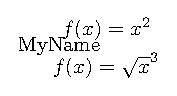
\includegraphics{../img/thelabel.eps}}
\end{figure}
%}}} end sec:picture

%{{{ sec:string
\section{string}
\index{Type-string}
\label{sec:string}

%}}} end sec:string

%{{{ sec:transform
\section{transform}
\index{Type-transform}
\label{sec:transform}

%}}}

%{{{ sec:color
\section{color}
\index{Type-color}
\label{sec:color}

\noindent\colortype{color}用于在执行绘图命令时使用\keyword{withcolor}进行改变颜色。\newline
\keyword{withcolor}接受\colortype{rgbcolor}时{\bf map to}\keyword{withrgbcolor}\newline
\keyword{withcolor}接受\colortype{cmykcolor}时{\bf map to}\keyword{withcmykcolor}\newline
\keyword{withcolor}接受\type{numberic}时{\bf map to}\keyword{withgreyscale}\newline
\keyword{withcolor}接受\constant{true}时{\bf map to}\other{current default color}\newline
\keyword{withcolor}接受\constant{false}时{\bf map to}\keyword{withoutcolor}\newline

\subsection{rgbcolor}
\index{Type-rgbcolor}
\label{subsec:rgbcolor}

\begin{mpostcode}[code:rgbcolorex]
    rgbcolor testrgb;
    testrgb:= 0.5red + 0.2green + 0.1blue;
    numeric colorpart[];
    colorpart1:=redpart testrgb;
    colorpart2:=greenpart testrgb;
    colorpart3:=bluepart testrgb;

    for i:=1 upto 3: show colorpart[i]; endfor;
\end{mpostcode}

\keyword{redpart},\keyword{greenpart},\keyword{bluepart}分别用于取得\colortype{rgbcolor}的 (r,g,b)。
\colortype{rgbcolor}的表达式:\newline
\expression{\lstinline$<rgbcolor>c := <numeric>*red + <numeric>*green + <numeric>*blue;$}%
或者\expression{\lstinline$<rgbcolor>c := (<numeric>, <numeric>, <numeric>)$}。
\index{Macro-redpart}\index{Macro-greenpart}\index{Macro-bluepart}

\subsection{cmykcolor}
\index{Type-cmdkcolor}
\label{subsec:cmykcolor}

\other{cmyk = cyan,magenta,yellow,black}\par

与\colortype{rgbcolor}类似的,也有\keyword{cyanpart},\keyword{magentapart},\keyword{yellowpart},%
\keyword{blackpart},表达式不能使用颜色相加的形式。\par
\begin{mpostcode}[code:cmyktest]
cmykcolor testcmyk;
    testcmyk:= (0.1, 0.2, 0.3, 0.4);
    numeric colorpart[];
    colorpart1:=cyanpart testcmyk;
    colorpart2:=magentapart testcmyk;
    colorpart3:=yellowpart testcmyk;
    colorpart4:=blackpart testcmyk;

    for i:=1 upto 4: show colorpart[i]; endfor;
\end{mpostcode}

\subsection{grey}
\label{subsec:grey}

\other{grey}使用\type{numeric}类型表示,范围{\bf [0,1]},从黑到白。
可以使用\macro{greypart}得到\other{grey}颜色的灰度。
\index{Macro-greypart}

%}}} end sec:color


\chapter{Expression}


\chapter{Equation}


\chapter{Control Folw}

\definecolor{relation}{rgb}{0.3, 0.8, 0.9}
\def\rel#1{{\color{relation} #1}}

关键字:\quad\keyword{else, elseif, endfor, exitif, fi, for, forever,%
    forsuffixes, if, step, until, beigngroup, endgroup}

%{{{ sec:condition
\section{Condition}
\index{Expr-condition}

\expression{if <bool expression>: $\ldots$ else: $\ldots$ fi}\quad 或者:\newline
\indent\expression{if <bool expression>: $\ldots$ elseif <bool expression>: $\ldots$ fi}\par

\fbox{\vbox{\moveright\parindent\vbox{\noindent
$\lag\text{\keyword{if}\ test}\rag\,\rightarrow\,\text{\keyword{if}}\lag\text{bool expression}%
\rag:\lag\text{balance tokens}\rag\lag\text{alternatives}\rag \text{\keyword{fi}}$\newline
$\lag\text{alternatives}\rag\,\rightarrow\,\lag\text{empty}\rag$\newline
\indent$|\text{\keyword{else}}:\lag\text{balance tokens}\rag$\newline
\indent$|\text{\keyword{elseif}}\lag\text{bool expression}\rag:\lag\text{balance tokens}\rag%
\lag\text{alternatives}\rag$
\footnote{Come from $\lag\text{{\bf METAPOST}\ a user's manual}\rag$}
}}}

\subsection{Bool Expression}
\label{sec:BoolExpression}
\index{Bool exression}

\fbox{\vbox{\moveright\parindent\vbox{\noindent
$\lag\text{bool primary}\rag\,\rightarrow\,\lag\text{bool variable}\rag$\newline
\indent$|\,\text{\constant{true}}\,|\,\text{\constant{false}}$\newline
\indent$|\,\left(\lag\text{boolean expression}\rag\right)$\newline
\indent$|\,\text{\keyword{begingroup}}\>\lag\text{statement list}\rag\lag\text{boolean expression}\rag%
\>\text{\keyword{endgroup}}$\newline
\indent$|\,\text{\keyword{known}}\>\lag\text{primary}\rag\,|\,\text{\keyword{unknown}}\lag%
\text{primary}\rag$\newline
\indent$|\,\lag\text{type}\rag\lag\text{primary}\rag\,|\,\text{\keyword{cycle}}\lag\text{primary}%
\rag$\newline
\indent$|\,\text{\keyword{odd}}\>\lag\text{numeric primary}\rag$\newline
\indent$|\,\text{\keyword{not}}\>\lag\text{boolean primary}\rag$\newline
$\lag\text{boolean secondary}\rag\,\rightarrow\,\lag\text{boolean primary}\rag$\newline
\indent$|\,\lag\text{boolean secondary}\rag\>\text{\keyword{and}}\>\lag\text{boolean primary}\rag$\newline
$|\lag\text{boolean tertiary}\rag\,\rightarrow\,\lag\text{boolean secondary}\rag$\newline
\indent$|\,\lag\text{boolean tertiary}\rag\>\text{\keyword{or}}\>\lag\text{boolean secondary}\rag$\newline
$\lag\text{boolean expression}\rag\,\rightarrow\,\lag\text{boolean tertiary}\rag$\newline
\indent$|\,\lag\text{numeric expression}\rag\lag\text{relation}\rag\lag\text{numeric tertiary}\rag$\newline
\indent$|\,\lag\text{pair expression}\rag\lag\text{relation}\rag\lag\text{pair tertiary}\rag$\newline
\indent$|\,\lag\text{transform expression}\rag\lag\text{relation}\rag\lag\text{transform tertiary}\rag$\newline
\indent$|\,\lag\text{boolean expression}\rag\lag\text{relation}\rag\lag\text{boolean tertiary}\rag$\newline
\indent$|\,\lag\text{string expression}\rag\lag\text{relation}\rag\lag\text{string tertiary}\rag$\newline
$\lag\text{relation}\rag\,\rightarrow\,\rel{<} | \rel{<=} | \rel{>} | \rel{>=} | \rel{=} | \rel{<>}$\par
}}}
%}}} end sec:condition

%{{{ sec:Loop
\section{Loop}
\index{Expr-Loop}

\begin{quote}
$\text{\keyword{for}}\,\lag\text{symbolic tokens}\rag=\lag\text{numeric expression}\rag%
\,\text{\keyword{step}}\,\lag\text{numeric}\rag\,\text{\keyword{until}}\,\lag\text{numeric}\rag:%
\,\text{loop text}\,\text{\keyword{endfor}}$

$\text{\keyword{for}}\,\lag\text{symbolic tokens}\rag=\lag\text{expression}\rag\,\text{\keyword{upto | downto}}:%
\lag\text{expression}\rag:\,\lag\text{loop text}\rag\,\text{\keyword{endfor}}$

$\text{\keyword{forsuffixes}}\,\lag\text{symbolic tokens}\rag=\text{suffix list}:\,\lag\text{loop text}\rag\,%
\text{\keyword{endfor}}$

$\text{\keyword{for}}\,\lag\text{symbolic tokens}\rag=\lag\text{picture expression}\rag:\,\lag\text}} end sec:loop

%{{{ sec:group
\section{group}
\index{Expr-group}
%}}} end sec:group


\chapter{Macro}

\section{无参宏}

\section{expr}

\section{text}

\section{suffix}


\chapter{Primary}


\backmatter

\printindex

\end{document}


%% \type for type keyword
%% \expression for expression
%% \colorexpr for color expression and color
%% \colortype for color type
%% \keyword for keyword
%% \marco for macro
%% \constant for internal variable
%% \unit for units
%% \number for number

%% {type:<type>} for the label of type
%% {Type-<type>} for the index of type
%% {expr:<expr} for the label of expr
%% {Expr-<expr>} for the index of expr
%% {macro:<marco>} for the label of macro
%% {Macro-<marco>} for the index of macro
%% {cons:<internal var>} for the label of internal variable
%% {Cons-<internal var>} for the index of internal variable
%% and so on.
%% define macro for this
